\chapter{Overview} \label{ch:OverView}
\chapterquote{Anything beyond your capacity will necessarily change your capacity, because so long as everything is within your limits, you don't know what is beyond them.}{Meher Baba}

\graphicspath{{Chapters/Overview/Figures/}}
\lstinputpath{Codes-Verilog/Chapter-Overview/VerilogCodes} %path is defined in mypreamble

\section{Introduction}
Verilog is the hardware description language which is used to model the digital systems. In this tutorial, following 4 elements of Verilog designs are discussed briefly, which are used for modeling the digital system.. 
\begin{enumerate}
	\item Design with Continuous assignment statements
	\item Structural design
	\item Design with Procedural assignment statements
	\item Mixed design
	
\end{enumerate}

The 2-bit comparators are implemented using various methods and corresponding designs are illustrated, to show the differences in these methods. Note that, all the features of Verilog can not be synthesized i.e. these features can not be converted into designs. Only, those features of Verilog are discussed in this tutorial, which can be synthesized.

%\href{https://www.altera.com/downloads/software/quartus-ii-we/111sp1.html}{`Quartus II 11.1sp1 Web Edition'} and \href{https://www.altera.com/downloads/software/modelsim-starter/111.html}{`ModelSim-Altera Starter'} softwares are used for this tutorial, which are freely available and can be downloaded from the \href{https://www.altera.com/downloads/download-center.html}{Altera website}. All the codes can be \href{http://pythondsp.readthedocs.io/en/latest/pythondsp/toc.html}{downloaded from the website}. First line of each listing in the tutorial, is the name of the Verilog file in the downloaded zip-folder. Also, see Appendix \ref{QuartusModelsim} to compile and synthesize the codes of the tutorial.

\section{Modeling styles} \label{sec:ModelingStyles}
In Verilog, the model can be designed in four ways as shown in this section. Two bit comparator is designed with different styles; which generates the output `1' if the numbers are equal, otherwise output is set to `0'.   

\subsection{Continuous assignment statements}
In this modeling style, the relation between input and outputs are defined using signal assignments. `assign' keyword is used for this purpose. In the other words, we do not define the structure of the design explicitly; we only define the relationships between the signals; and structure is implicitly created during synthesis process. 

\begin{explanation}[Listing \ref{verilog:andEx}]
	Listing \ref{verilog:andEx} is the example of `Continuous assignment statements' design, where relationship between inputs and output are given in line 8. In verilog, `$\&$' sign is used for `and' operation (line 8), and `$//$' is used for comments (line 1). The `and gate' generated by Listing \ref{verilog:andEx} is shown in \ref{fig:andEx}. 
	\\ \\
	Note that, in lines 4 and 5, `wire' keyword is used which is the `data type'. For continuous assignment statements `wire' keyword is used; whereas `reg' keyword is used for procedural assignment statement. Further, input ports can not be defined as `reg'. Note that, these keyword are not interchangeable and the differences between these `data types' are discussed in section \ref{sec:proceduralModeling}. Further, more operators e.g. `and', `not' and `nand' etc. are discussed in Chapter \ref{ch:Datatypes}. 
\end{explanation}

\lstinputlisting[
language = Verilog,
caption    = {And gate},
label      = {verilog:andEx}
]{andEx.v}

\begin{figure}[!h]
	\centering
	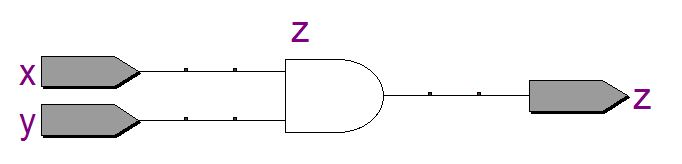
\includegraphics[scale=0.3]{andEx}
	\caption{And gate, Listing \ref{verilog:andEx}}
	\label{fig:andEx}
\end{figure}

Listing \ref{verilog:andEx} can be written as Listing \ref{verilog:andEx2}, where module-definition contains name of ports only (Line 3); and types of ports are defined outside the module (Lines 5-6). 
\lstinputlisting[
language = Verilog,
caption    = {And gate},
label      = {verilog:andEx2}
]{andEx2.v}

\subsection{Comparators using Continuous assignment statements}

In this section, two more examples of Continuous assignment statements are shown i.e. `1 bit' and `2 bit' comparators; which are used to demonstrate the differences between various modeling styles in the tutorial. Table \ref{tbl:comparator1Bit} and \ref{tbl:comparator2Bit} show the truth tables of `1 bit' and `2 bit' comparators.  As the name suggests, the comparator compare the two values and sets the output `eq' to 1, when both the input values are equal; otherwise `eq' is set to zero. The corresponding boolean expressions are shown below, 

\begin{table}[!h]
	\centering
	\caption{1 bit comparator, Listing \ref{verilog:comparator1Bit}}
	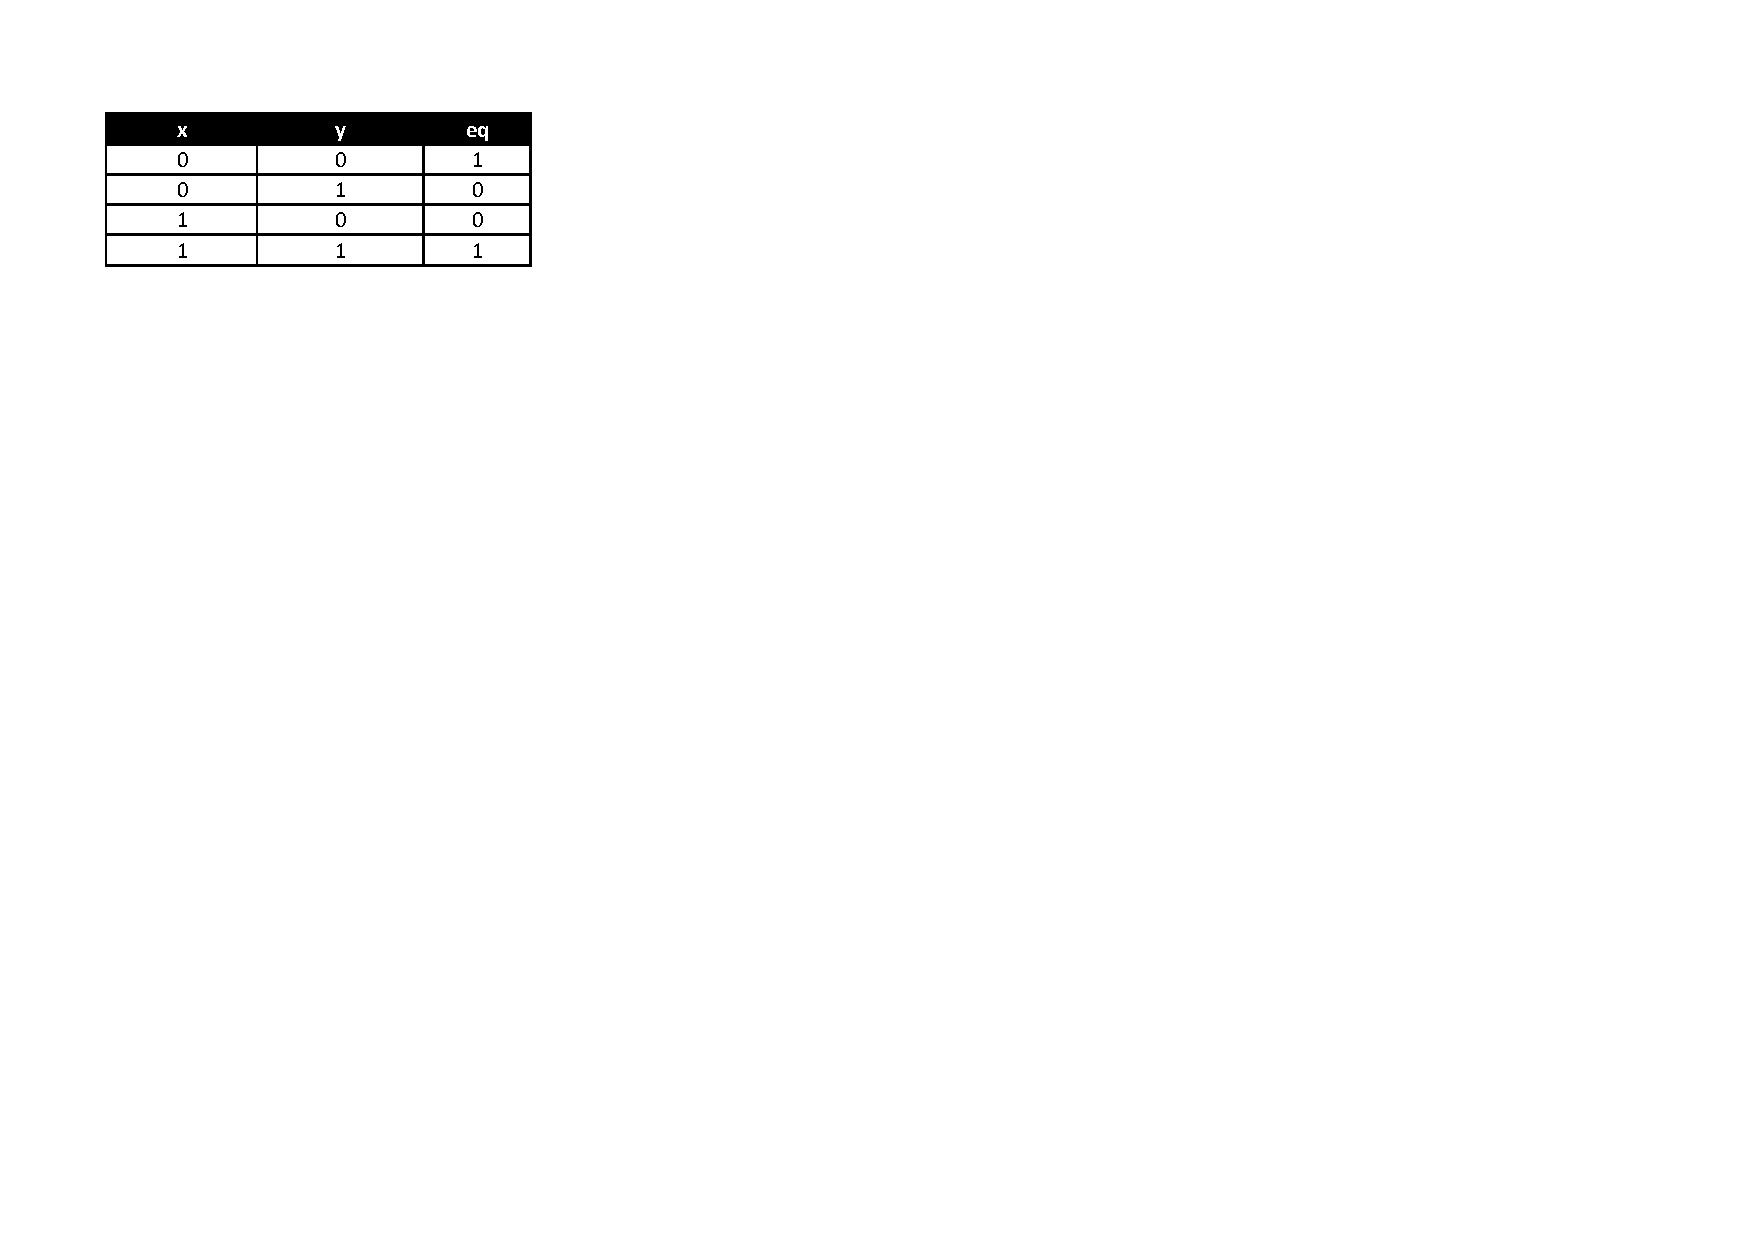
\includegraphics[scale=0.7]{TableComparator1Bit}
	\label{tbl:comparator1Bit}
\end{table}

\begin{table}[!h]
	\centering
	\caption{2 bit comparator, Listing \ref{verilog:comparator2Bit}}
	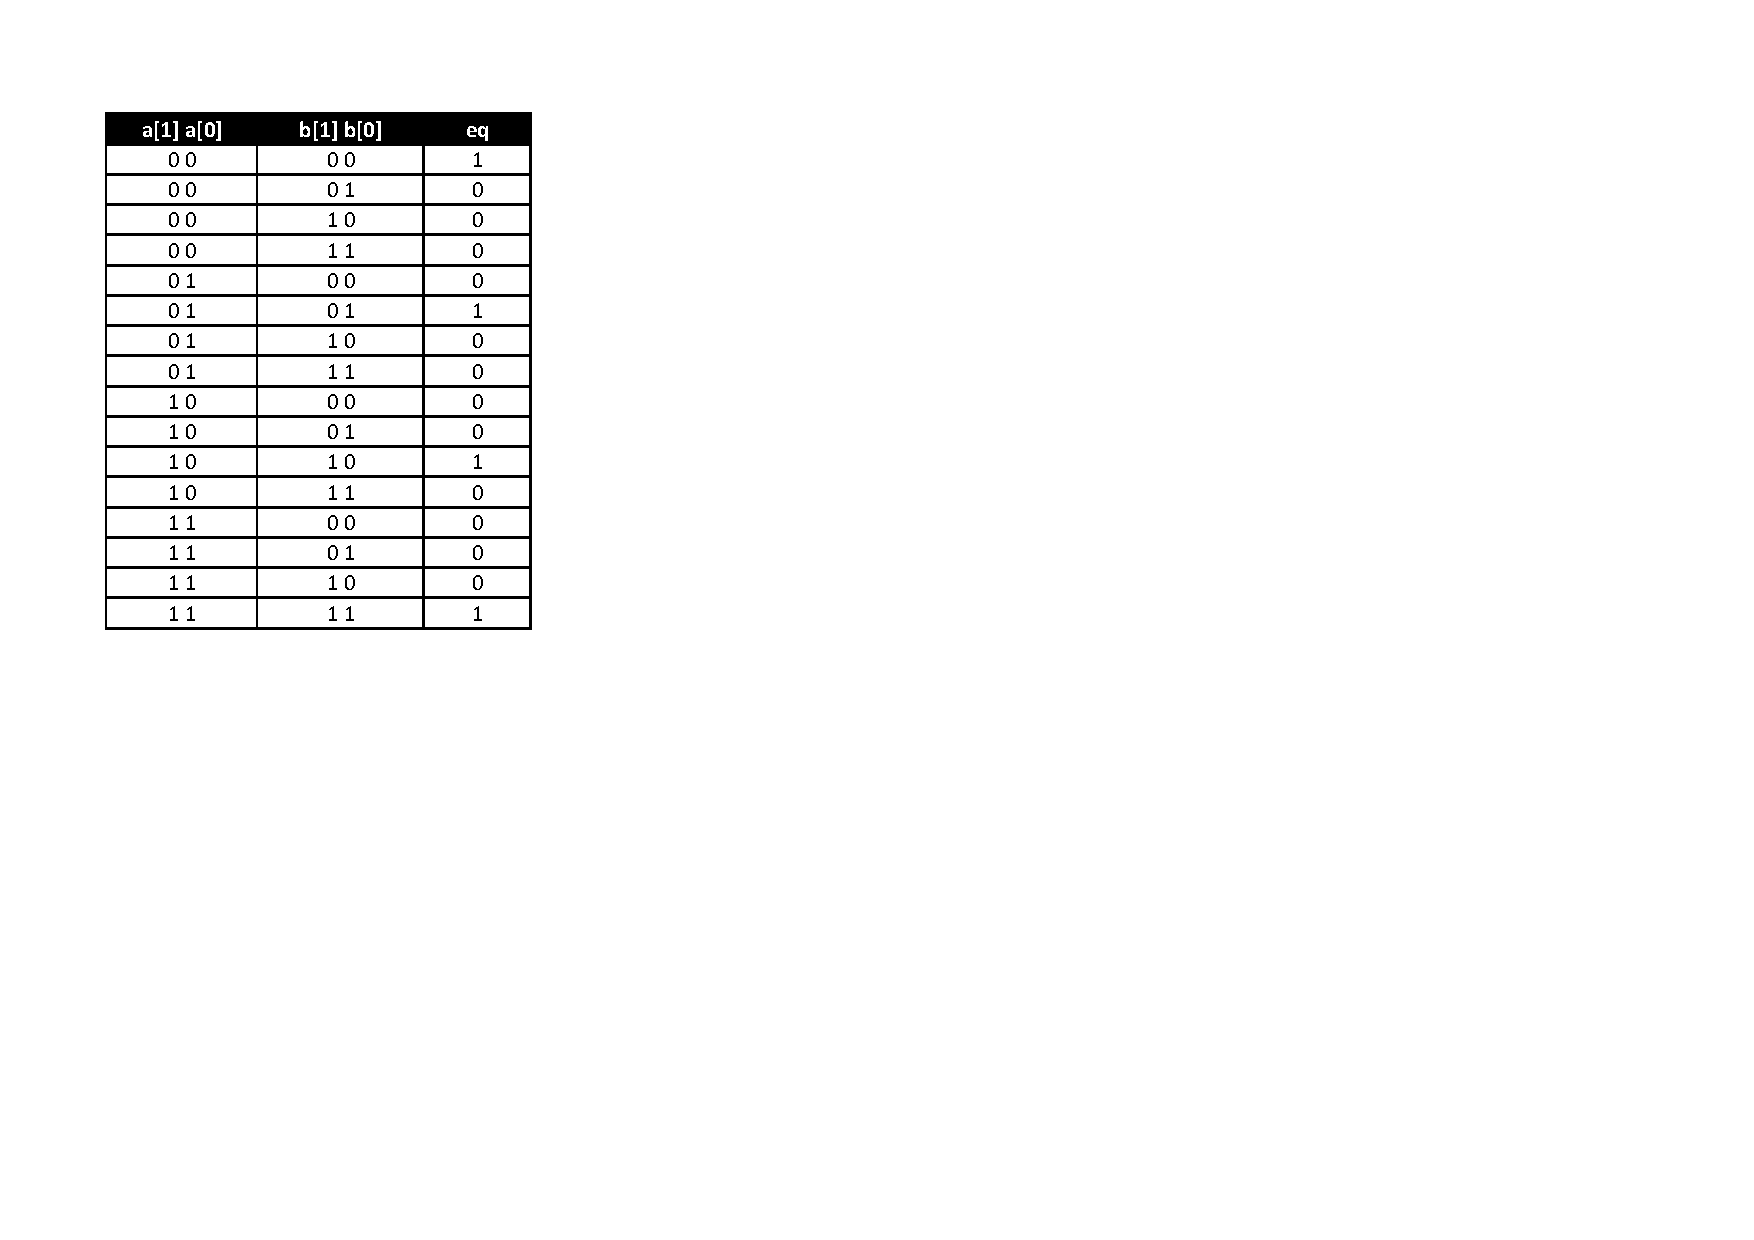
\includegraphics[scale=0.7]{TableComparator2Bit}
	\label{tbl:comparator2Bit}
\end{table}

For 1 bit comparator: 
\begin{equation}
eq = x' y' + x y
\label{eq:1bitComparator}
\end{equation} 

For 2 bit comparator: 
\begin{equation}
eq = a'[1]a'[0]b'[1]b'[0] + a'[1]a[0]b'[1]b[0] + a[1]a'[0]b[1]b'[0] + a[1]a[0]b[1]b[0]
\label{eq:2bitComparator}
\end{equation} 
Above two expressions are implemented using verilog in Listing \ref{verilog:comparator1Bit} and \ref{verilog:comparator2Bit}, which are explained below.

\begin{explanation}[Listing \ref{verilog:comparator1Bit}: 1 bit comparator]
	Listing \ref{verilog:comparator1Bit} implements the 1 bit comparator based on equation \ref{eq:1bitComparator}. Two intermediate signals are defined in line 8. These two signals ($s0$ and $s1$) are defined to store the values of $x'y'$ and $xy$ respectively. Values to these signals are assigned at line 10 and 11. In verilog, `not' and `or' operations are implemented using `$\sim$' and `$|$' signs as shown in line 10 and 12 respectively. Finally equation \ref{eq:1bitComparator} performs `or' operation on these two signals, which is done at line 12. When we compile this code using `Quartus software', it implements the code into hardware design as shown in Fig. \ref{fig:comparator1Bit}.
	
	The compilation process to generate the design is shown in Appendix \ref{QuartusModelsim}. Also, we can check the input-output relationships of this design using Modelsim, which is also discussed briefly in Appendix \ref{QuartusModelsim}.   
\end{explanation}
\lstinputlisting[
language = Verilog,
caption    = {Comparator 1 Bit},
label      = {verilog:comparator1Bit}
]{comparator1Bit.v}


\begin{noNumBox}
	Note that, the statements in `Continuous assignment statements' and `structural modeling' (described in section \ref{sec:structureModeling}) are the concurrent statements, i.e. these statements execute in parallel. In the other words, order of statements do not affect the behavior of the circuit; e.g. if we exchange the lines 10, 11 and 12 in Listing \ref{verilog:comparator1Bit}, again we will get the Fig. \ref{fig:comparator1Bit} as implementation. 
	
	On the other hand, statements in `Procedural assignment statements' (described in section \ref{sec:proceduralModeling}) executes sequentially and any changes in the order of statements will change the behavior of circuit. 
\end{noNumBox}
%
\begin{explanation}[Fig. \ref{fig:comparator1Bit}: 1 bit comparator]
	Fig. \ref{fig:comparator1Bit} is generated by Quartus software according to the verilog code shown in Listing \ref{verilog:comparator1Bit}. Here, $s0$ is the `and' gate with inverted inputs $x$ and $y$, which are generated according to line 10 in Listing \ref{verilog:comparator1Bit}. Similarly,  $s1$ `and' gate is generated according to line 11. Finally output of these two gates are applied to `or' gate (named as `eq') which is defined at line 12 of the Listing \ref{verilog:comparator1Bit}.   
\end{explanation}
\begin{figure}[!h]
	\centering
	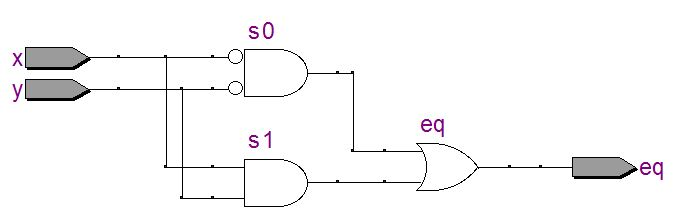
\includegraphics[scale=0.4]{comparator1Bit}
	\caption{ 1 bit comparator, Listing \ref{verilog:comparator1Bit}}
	\label{fig:comparator1Bit}
\end{figure}
%
\begin{explanation}[Listing \ref{verilog:comparator2Bit}: 2 bit comparator] 
	This listing implements the equation \ref{eq:2bitComparator}. Here, we are using two bit input, therefore `wire[1:0]' is used at line 4. `1:0' sets the 1 as MSB (most significant bit) and 0 as LSB(least significant bit) i.e. the $a[1]$ and $b[1]$ are the MSB, whereas $a[0]$ and $b[0]$ are the LSB. Since we need to store four signals (lines 10-13), therefore `s' is defined as 4-bit vector in line 8. Rest of the working is same as Listing \ref{verilog:comparator1Bit}. The implementation of this listing is shown in Fig. \ref{fig:comparator2Bit}. 
\end{explanation}
\lstinputlisting[
language = Verilog,
caption    = {Comparator 2 Bit},
label      = {verilog:comparator2Bit}
]{comparator2Bit.v}
\begin{figure}[!h]
	\centering
	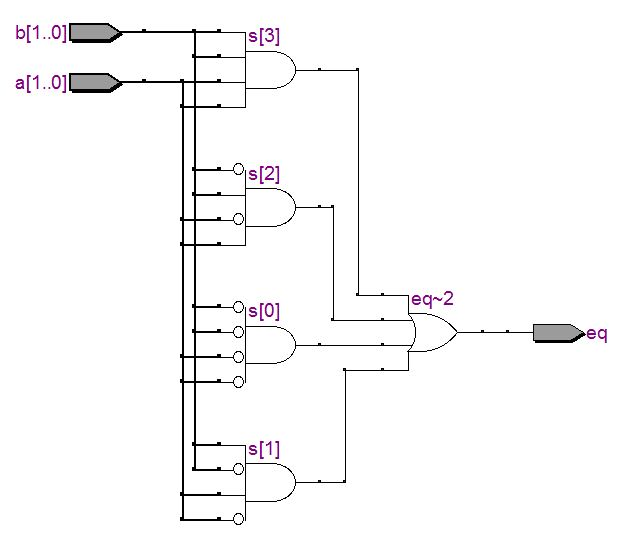
\includegraphics[scale=0.45]{comparator2Bit}
	\caption{2 bit comparator, Listing \ref{verilog:comparator2Bit}}
	\label{fig:comparator2Bit}
\end{figure}
%

\subsection{Structural modeling}\label{sec:structureModeling}
In previous section, we designed the 2 bit comparator based on equation \ref{eq:2bitComparator}. Further, we can design the 2 bit comparator using 1-bit comparator as well, with following steps, 
\begin{enumerate}
	\item First compare each bit of 2-bit numbers using 1-bit comparator;  i.e. compare $a[0]$ with $b[0]$ and $a[1]$ with $b[1]$ using 1-bit comparator (as shown in Table \ref{tbl:comparator2Bit}). 
	
	\item If both the values are equal, then set the output `eq' as 1, otherwise set it to zero. 
\end{enumerate}

This method is known as `structural' modeling, where we use the pre-defined designs to create the new designs (instead of implementing the `boolean' expression). This method is quite useful, because most of the large-systems are made up of various small design units. Also, it is easy to create, simulate and check the various small units instead of one large-system. Listing \ref {verilog:comparator2BitStruct} is the example of structural designs, where 1-bit comparator is used to created a 2-bit comparator.  

\begin{explanation}[Listing \ref{verilog:comparator2BitStruct}]
	In this listing, lines 4-5 define the two input ports of 2-bit size and one 1-bit output port. Then two signals are defined (line 8) to store the outputs of two 1-bit comparators, as discussed below.
	
	`$eq\_bit0$' and `$eq\_bit1$' in lines 10 and 11 are the names of the two 1-bit comparator, which are used in this design. We can see these names in the resulted design, which is shown in Fig. \ref{verilog:comparator2BitStruct}.  
	
	Next, `comparator1Bit' in lines 10 and 11 is the name of the 1-bit comparator (defined in Listing \ref{verilog:comparator1Bit}). With this declaration, i.e. comparator1bit, we are calling the design of 1-bit comparator to current design. 
	
	Then, mapping statements e.g. $.x(a[0])$ in lines 10 and 11, are assigning the values to the input and output port of 1-bit comparator. For example, in line 10, input ports of 1-bit comparator i.e. $x$ and $y$, are assigned the values of $a[0]$ and $b[0]$ respectively from this design; and the output $y$ of 1-bit comparator is stored in the signal $s0$. Further, in line 13, if signals $s0$ and $s1$ are 1 then `eq' is set to 1 using `and' gate, otherwise it will be set to 0. Final design generated by Quartus software for Listing \ref{verilog:comparator2BitStruct} is shown in Fig. \ref{fig:comparator2BitStruct}. 
\end{explanation}

\lstinputlisting[
language = Verilog,
caption    = {Structure modeling using work directory},
label      = {verilog:comparator2BitStruct}
]{comparator2BitStruct.v}
\begin{figure}
	\centering
	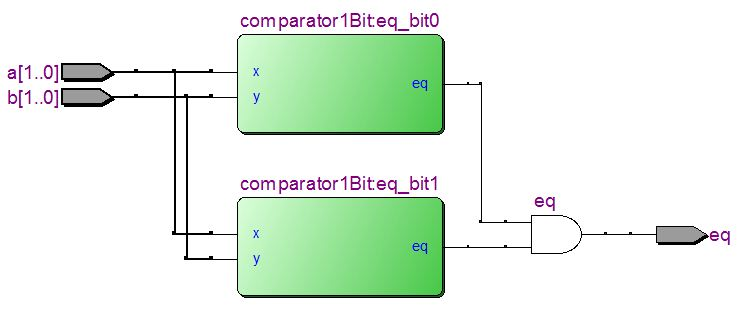
\includegraphics[scale=0.5]{comparator2BitStruct}
	\caption{2 bit comparator, Listing \ref{verilog:comparator2BitStruct}}
	\label{fig:comparator2BitStruct}
\end{figure}

\begin{explanation}[Fig. \ref{fig:comparator2BitStruct}]
	In this figure, a[1..0] and b[1..0]  are the input bits  whereas `eq' is the output bit. Thick lines after a[1..0] and b[1..0] show that there are more than 1 bits e.g. in this case these lines have two bits. These thick lines are changed to thin lines before going to comparators; which indicates that only 1 bit is sent as input to comparator. 
	
	In `comparator1Bit: eq\_bit0', `comparator1Bit' is the name of the module defined for 1-bit comparator (Listing \ref{verilog:comparator1Bit}); whereas the `eq\_bit0' is the name of this module defined in line 10 of listing \ref{verilog:comparator2BitStruct}. Lastly outputs of two 1-bit comparator are sent to `and' gate according to line 13 in listing \ref{verilog:comparator2BitStruct}. 
	
	Hence, from this figure we can see that the 2-bit comparator can be designed by using two 1-bit comparator. 
\end{explanation}

\subsection{Procedural assignment statements}\label{sec:proceduralModeling}
In Procedural assignment statements, the `always' keyword is used and all the statements inside the always statement execute sequentially. Various conditional and loop statements can be used inside the process block as shown in Listing \ref{verilog:comparator2BitProcedure}. Further, always blocks are concurrent blocks, i.e. if the design has multiple always blocks (see Listing \ref{verilog:comparator2BitMixed}), then all the always blocks will execute in parallel. 

\begin{explanation}[Listing \ref{verilog:comparator2BitProcedure}: Procedural assignment statement]
	The `always' block is declared in line 8, which begins and ends at line 9 and 14 respectively. Therefore all the statements between line 9 to 14 will execute sequentially and Quartus Software will generate the design based on the sequences of the statements.  Any changes in the sequences will result in different design.
	
	Note that, the output port `eq' is declared as \textbf{reg} at line 5. If we assign value to the signal inside the `always' block then that signal must be declared as `reg' e.g. value of `eq' is assigned in line 11 and 13, which are inside the `always' block; hence `eq' is declared as reg. 
	
	The `always' keyword takes two arguments in line 8 (known as `sensitivity list'), which indicates that the process block will be executed if and only if there are some changes in `a' and `b'. `@' is used after `always' for defining the sensitivity list. In line 10-13, the `if' statement is declared which sets the value of `eq' to 1 if both the bits are equal (line 10-11), otherwise `eq' will be set to 0 (line 12-13). Fig. \ref{fig:comparator2BitProcedure} shows the design generated by the Quartus Software for this listing. `==' in line 10 is one of the condition operators; whereas $\&\&$ is the logical operator, which are discussed in detail in Chapter \ref{ch:Datatypes}.
\end{explanation}
\lstinputlisting[
language = Verilog,
caption    = {Procedural assignment statement},
label      = {verilog:comparator2BitProcedure}
]{comparator2BitProcedure.v}
\begin{figure}
	\centering
	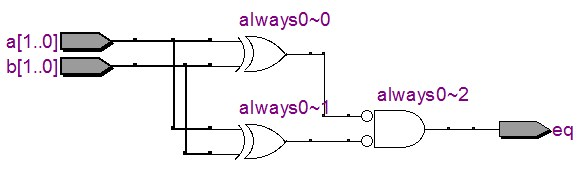
\includegraphics[scale=0.5]{comparator2BitProcedure}
	\caption{2 bit comparator, Listing \ref{verilog:comparator2BitProcedure}}
	\label{fig:comparator2BitProcedure}
\end{figure}

\subsection{Mixed modeling}
We can mixed all the modeling styles together as shown in Listing \ref{verilog:comparator2BitMixed}. Here two always blocks are used in line 10 and 18, which is the `procedural assignment statements'. Then in line 26, `continuous assignment statement' is used for assigning the value to output variable `eq'.

\begin{explanation}[Listing \ref{verilog:comparator2BitMixed}: Mixed modeling]
	Note that, output `eq' is defined as `wire' (as value to `eq' is assigned using continuous assignment statement), whereas signals `s0' and `s1' is defined as `reg' (as values are assigned using procedural assignment statement i.e. inside the `always' block). Two always blocks are used here. Always block at line 10 checks whether the LSB of two numbers are equal or not; if equal then signal `s0' is set to 1 otherwise it is set to 0. Similarly, the always block at line 18, sets the value of `s1' based on MSB values. Lastly, line 16 sets the output `eq' to 1 if both `s0' and `s1' are 1, otherwise it is set to 0. The design generated for this listing is shown in Fig. \ref{fig:comparator2BitMixed}.
\end{explanation}
\lstinputlisting[
language = Verilog,
caption    = {Multiple procedural assignment statements},
label      = {verilog:comparator2BitMixed}
]{comparator2BitMixed.v}
\begin{figure}
	\centering
	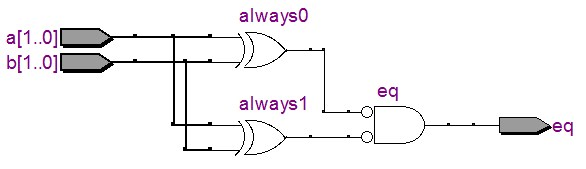
\includegraphics[scale=0.5]{comparator2BitMixed}
	\caption{2 bit comparator, Listing \ref{verilog:comparator2BitMixed}}
	\label{fig:comparator2BitMixed}
\end{figure}
%

\section{Conclusion}
In this tutorial, various features of Verilog designs are discussed briefly. We designed the two bit comparator with four modeling styles i.e. Continuous assignment statement, Structural design, Procedural assignment statement and Mixed styles. Also, differences between the generated-designs with these four methods are shown.